\documentclass[11pt,ngerman,parskip=half]{scrartcl}

\usepackage[utf8]{inputenc}
\usepackage[T1]{fontenc}
\usepackage{libertine}
\usepackage{babel}
\usepackage{graphicx}
\usepackage[style=authoryear-icomp,dashed=false,loccittracker=context]{biblatex}
\usepackage[thresholdtype=lines,threshold=2]{csquotes}
\usepackage{xpatch}
%\usepackage{hyperref}
\usepackage{float}
\usepackage{url}
\usepackage{paralist}

\setlength\bibitemsep{1.5\itemsep}
\urlstyle{same}
\addbibresource{src/library.bib}
\author{}
\titlehead{
  \begin{center}
     
\includegraphics[width=0.7\textwidth]{src/img/htw-logo.pdf}
  \end{center}
}
\title{Gehirn-Computer-Schnittstellen in Neuroprothesen}

\begin{document}
\maketitle
\begin{tabular}{ll}
  Fachbereich: & 4 (Informatik, Kommunikation und Wirtschaft) \\
  Studiengang: & Angewandte Informatik (SoSe2018)             \\
  Seminar:     & B15 Gesellschaftliche Aspekte der Informatik \\
  Dozentin:    & Prof.-Dr. Christin Schmidt                   \\
\end{tabular}

\begin{tabular}{ll}
  Gruppe: & 5 \\
\end{tabular}

\begin{tabular}{lll}
  Gruppenmitglied        & Matrikelnummer & Kapitel\\
  Louis Knorn            & 566546         & 1\\
  John-Kevin Gold        & 566538         & 2\\
  Jeremy Etienne Seipelt & 566847         & 3\\
  Kathrin Klocke         & 514403         & 4\\
\end{tabular}

\newpage
\tableofcontents
\newpage
\listoffigures
\newpage
\listoftables
\newpage

\section{Funktionsweise der Gerätetechnik von Gelenkarmrobotern}
\label{sec:john}
\subsection{Einführung}
\label{subsec:john_einfuehrung}
Der Artikel \enquote{Neuroprothese: Gelähmter steuert Roboterarm mit bloßer
Vorstellungskraft} aus dem Jahr 2015 beschreibt, wie ein Mensch einen
Industrieroboter-ähnlichen Gelenk- bzw. Knickarmroboter mittels eines
Brain-Computer-Interface steuert
\parencite[vgl.][]{merkelt_neuroprothesen:_2015}. Die Idee, verlorene oder
gelähmte Gliedmaßen durch Roboterarme zu ersetzen, ist allerdings nicht völlig
neu. Bereits im Jahr 1979 veröffentlichten Guittet u. a. eine Fallstudie, die
eine vergleichbare Anwendung untersuchte. Man bezeichnete einen solchen
Roboterarm auch als Telethese, allerdings wurde der Arm damals durch einfache
Kopfbewegungen kontrolliert \parencite[vgl.][]{guittet_spartacus_1979}.

\begin{figure}[H]
  \centering
  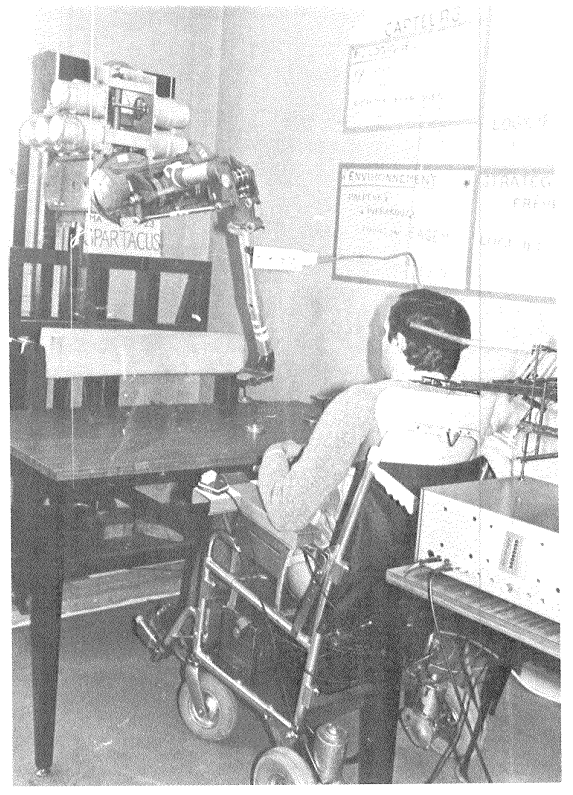
\includegraphics[width=0.6\textwidth]{src/img/john1.png}
  \caption{Knickarmrobotersteuerung durch Kopfbewegungen}
  \label{img:john1}
  \parencite[][84]{guittet_spartacus_1979}
\end{figure}
\newpage

Nachdem im ersten Kapitel der Gruppenarbeit die Funktionsweise von BCI
erläutert wurde, beschäftigt sich der folgende Abschnitt mit der
Gerätetechnik eines Gelenkarmoboters sowie Begriffen und Grundlagen der
Robotik im Allgemeinen. Die Gerätetechnik gehört zu den Kernkomponenten in
einem Robotersystem und beinhaltet technische Elemente für Kinematik,
Sensorik und Aktorik. Zu den weiteren Kernkomponenten, die im Rahmen der
Belegarbeit nicht weiter behandelt werden, zählen:
\begin{compactitem}
  \item Steuerung (z.B. Rechnerkopplung, Interpolation)
  \item Programmierung (z.B. Punkt- und Bahnsteuerung, Prozessbeschreibung)
  \item Prozessführung (Geometrie- und Technologiedatenverarbeitung, Steuer-
        und Regelstrategie)
  \item Endeffektor (z.B. Greifer, Werkzeuge)
\end{compactitem}
\parencite[vgl.][40]{hesse_taschenbuch_2016}

Der Begriff Robotik ist laut DIN definiert als:
\blockquote[{\cite[DIN EN ISO 8373, zitiert nach][39]
{hesse_taschenbuch_2016}}]{Robotertechnik, zu der man Entwurf und
Berechnung, Herstellung, Steuerung von Robotern, Einsatz in Standard- und
Problemlösungen, Erforschung von Steuerungsvorgängen bei Mensch und Maschine,
Sensoren und Endeffektoren sowie deren Anwendung zählt}.
Roboter können nach verschiedenen Kriterien, wie Anwendungsbereich,
Einsatzgebiet, Ausführung und Aufgaben, gruppiert werden
\parencite[vgl.][25\psq]{hesse_taschenbuch_2016}. Die VDI-Richtlinie 2860
beschreibt Industrieroboter beispielsweise wie folgt:
\blockquote[{\cite[VDI-Richtlinie 2860, zitiert nach][16]
{weber_industrieroboter:_2017}}]{Industrieroboter sind universell
einsetzbare Bewegungsautomaten mit mehreren Achsen, deren Bewegungen
hinsichtlich Bewegungsfolge und Wegen bzw. Winkeln frei programmierbar (d.h.
ohne mechanischen Eingriff vorzugeben bzw. änderbar) und gegebenenfalls
sensorgeführt sind. Sie sind mit Greifern, Werkzeugen oder anderen
Fertigungsmitteln ausrüstbar und können Handhabe- oder andere
Fertigungsaufgaben ausführen}.

Roboter, insbesondere Industrieroboter, können demnach auch als
Handhabungsgeräte bzw. -technik betrachtet werden.
Abbildung~\ref{img:john2} zeigt, dass
Handhabungsgeräte primär in manuell gesteuerte oder programmgesteuerte Geräte
eingeteilt werden können. Es gibt darüber hinaus aber auch Mischformen in der
Robotik, z.B. beim Serviceroboter. Dieser ist ein Hybrid aus Industrieroboter
und Manipulator, welcher Dienstleistungen für den Menschen erbringt.
Serviceroboter reagieren auf menschliche Anweisungen (manuelle Steuerung)
führen Teilaufgaben aber auch automatisch bzw. programmgesteuert aus.
\parencite[vgl.][15--17]{weber_industrieroboter:_2017}

\begin{figure}[H]
  \centering
  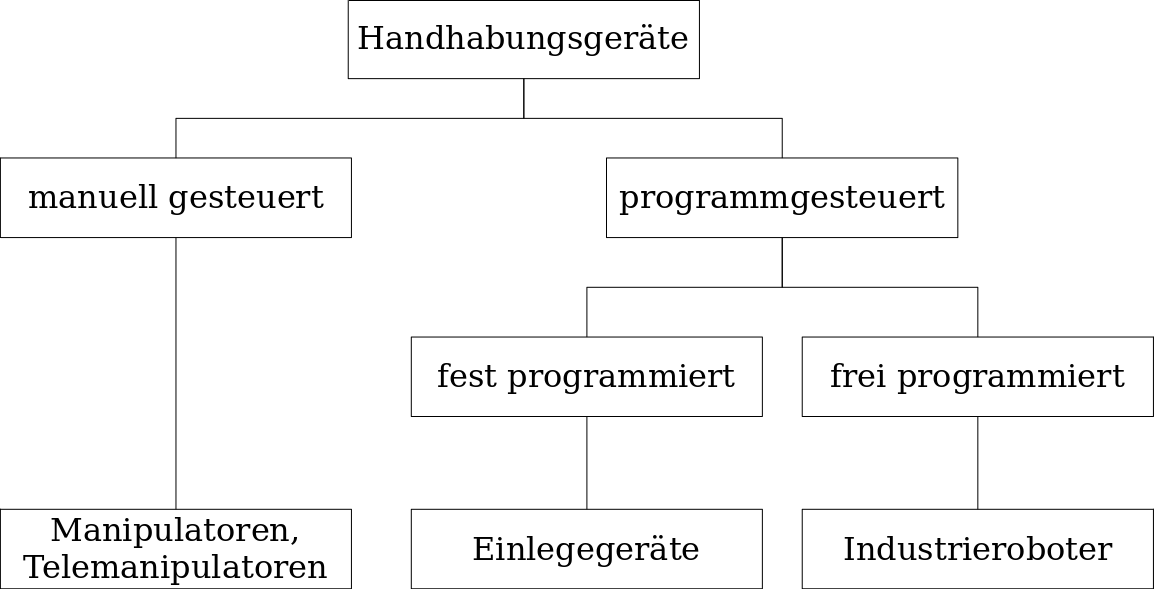
\includegraphics[width=0.7\textwidth]{src/img/john2.png}
  \caption{Einteilung von Handhabungsgeräten}
  \label{img:john2}
  \parencite[][16]{weber_industrieroboter:_2017}
\end{figure}

\subsection{Kinematik}
\label{subsec:john_kinematik}
Die Anordnung der Armteile und Gelenke bestimmt die kinematische Struktur
eines Roboters, hierbei unterscheidet man hauptsächlich zwischen serieller
Kinematik und Parallelkinematik. Roboter die aus einer Aneinanderreihung von
Armteilen bestehen, welche wiederum durch Gelenke bzw. Achsen verbunden sind,
ordnet man der seriellen Kinematik zu. Das letzte Armteil in einer solchen
Anordnung, kann auch als Effektor bzw. Endeffektor bezeichnet werden. Hierbei
handelt es sich um das Teil des Roboters, welches in Kontakt mit der Umgebung
tritt, um z.B. Objekte zu greifen. Bei der Parallelkinematik hingegen sind
mehrere Schub- oder Drehgelenke mit dem Effektor verbunden und wirken direkt
auf diesen. Der Gelenkarmroboter weist eine serielle Kinematik auf. Die
kinematische Struktur eines Roboters bestimmt wiederum seinen Freiheits- bzw.
Getriebefreiheitsgrad. \parencite[vgl.][17--20]{weber_industrieroboter:_2017}

Der Freiheitsgrad \textit{f} beschreibt
\textquote[{\cite[][18]{weber_industrieroboter:_2017}}]{[...] die Anzahl der
möglichen unabhängigen Bewegungen (Verschiebungen, Drehungen) eines starren
Körpers gegenüber einem Bezugssystem}. Es gibt hierbei zwei wesentliche
Grundbewegungen, die Translation (Gleit- oder Verschiebebewegung) und die
Rotation (Drehbewegung). Bei der Translation bewegt sich der Körper
theoretisch ohne sich selbst zu drehen (starr) entlang einer oder mehrerer
Raumachsen (x-, y- und z-Achse). Bei der Rotation hingegen dreht sich der
Körper um einen bestimmten Mittelpunkt bzw. um eine bestimmte Achse, die
innerhalb oder außerhalb des Körpers liegen kann.
\parencite[vgl.][53\psq]{schunke_funktionelle_2014}

Abbildung~\ref{img:john3} stellt die Freiheitsgrade am
Beispiel der Bewegungsmöglichkeiten eines Tennisballs im Raum dar.
\begin{figure}[H]
  \centering
  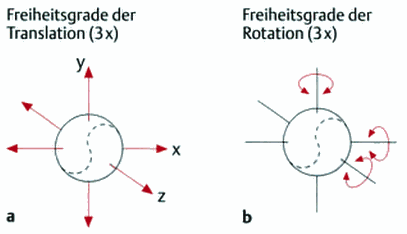
\includegraphics[width=0.6\textwidth]{src/img/john3.png}
  \caption{Translation (a) und Rotation (b)}
  \label{img:john3}
  \parencite[][53]{schunke_funktionelle_2014}
\end{figure}

Der Getriebefreiheitsgrad F gibt an,
\textquote[{\cite[][18]{weber_industrieroboter:_2017}}]{[...] wie viele
unabhängig voneinander angetriebene Achsen zu einer eindeutigen Bewegung des
Roboterarms führen}. Bei Gelenkarmrobotern mit sechs Achsen (F=6), kann der
Effektor durch geschickte Anordnung der Gelenke, den maximalen Freiheitsgrad
f=6 erreichen. Roboter können generell aber auch mit mehr als sechs Achsen
(F>6) konstruiert werden, dies bezeichnet man als redundante Kinematiken.
Hierdurch erzielt man auf Kosten eines erhöhten Steuerungsaufwands eine
Verbesserung der Feinbewegungen.
\parencite[vgl.][18]{weber_industrieroboter:_2017}

Abbildung~\ref{img:john4} zeigt die Drehrichtung der Roboterachsen des
Gelenkroboters KUKA KR AGILUS sixx.
\begin{figure}[H]
  \centering
  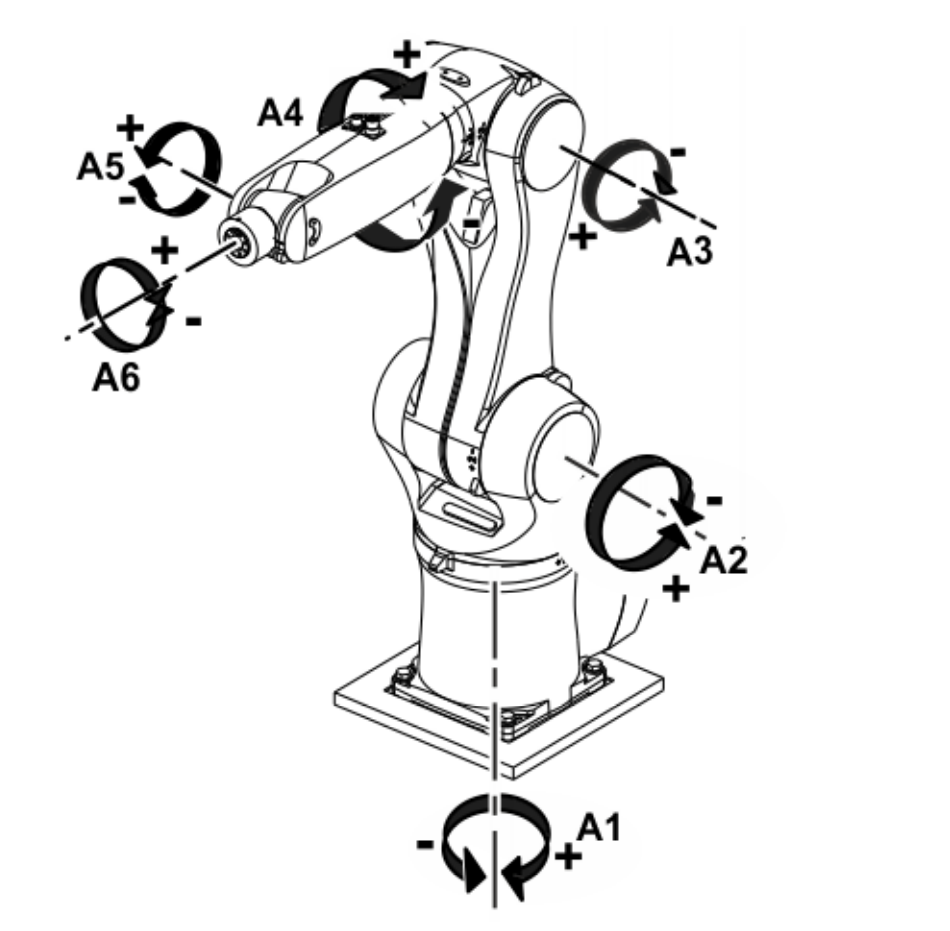
\includegraphics[width=0.5\textwidth]{src/img/john4.png}
  \caption{KR AGILUS sixx}
  \label{img:john4}
  \parencite{kuka_gmbh_kr_2018}
\end{figure}

\subsection{Aktorik}
\label{subsec:john_aktorik}
Gelenkmodule und Achsverbindungen werden durch die Aktorik eines Roboters
angetrieben und ermöglichen somit die Bewegung des Effektors. Der Aktor hat
demnach die Aufgabe eine Achse von einer Position auf eine andere zu bewegen,
hierzu gibt es vier typische Betriebszustände:
\begin{compactitem}
  \item Antrieb und Beschleunigung im Rechtslauf
  \item Abbremsung im Rechtslauf
  \item Antrieb und Beschleunigung im Linkslauf
  \item Abbremsung im Linkslauf
\end{compactitem}

Zu den wesentlichen Gruppen in der Aktorik gehören pneumatische oder
hydraulische Aktoren (z.B. doppeltwirkende Zylinder oder Druckluftmotoren)
sowie elektrische Aktoren (z.B. bürstenbehaftete und bürstenlose
Gleichstrommaschinen). Jede Gruppe hat ihre individuellen Vor- und Nachteile,
weshalb in einem Robotersystem, und so z.B. auch bei einem Gelenkarmroboter,
verschiedene Kombinationen von Aktoren zum Einsatz kommen können. Generell
lässt sich festhalten, dass pneumatische und hydraulische Aktoren die
höchsten Kräfte erzielen und daher sehr hohe Geschwindigkeiten erreichen
können, allerdings erreichen sie nicht die hohe Positioniergenauigkeit von
elektrischen Aktoren.
\parencite[vgl.][63--79]{hesse_taschenbuch_2016}

Neben dem eigentlichen Antrieb bzw. Motor sind auch Getriebe teil der Aktorik
in einem Roboter. Getriebe sind notwendig, da die Bewegungen der Aktoren
nicht immer direkt den Anforderung des mechatronischen Systems entsprechen.
Sie dienen allgemein der Übertragung und Umformung von Bewegungen sowie von
Kräften, mittels der Änderung von Drehmomenten, -richtungen oder der
Umsetzung einer Drehbewegung in eine Linearbewegung. Auch hier gibt es viele
verschiedene Bauformen, deren Anwendung je nach Anforderung variiert, z.B.
Kugelumlaufspindeln, Planetengetriebe, Kegelradgetriebe oder Zahnriemengetriebe.
\parencites[vgl.][121\psq]{maccloy_robotertechnik:_1989}
[][89--96]{hesse_taschenbuch_2016}

\subsection{Sensorik}
\label{subsec:john_sensorik}
Die Sensorik in einem Robotersystem ermittelt inner- und außerhalb des
Systems vorliegende Informationen. Dies ist erforderlich um die komplexen
Bewegungsabläufe in einer nur teilweise bestimmbaren Umwelt auszuführen. Die
Robotik stützt sich dabei häufig auf Erkenntnisse aus der Bionik\footnote{
Die Bionik erforscht wie biologische Phänomene auf technische Systeme
übertragen werden können. \parencite{feess_definition:_2018}} und man
unterscheidet primär zwischen internen (interozeptiven bzw. propriozeptiven)
und externen (exterozeptiven) Sensoren. Interozeptive Sensoren messen interne
Zustände wie Motorgeschwindigkeit, Ladezustand oder Greifkraft und
exterozeptive Sensoren ermitteln Informationen aus der Umgebung, z.B. zur
Entfernungsmessung von Objekten. Nutzt ein Sensor dabei nur die Energie bzw.
Signale aus der Umgebung, bezeichnet man ihn auch als passiven Sensor (z.B.
Kameras oder Kontaktsensoren). Aktive Sensoren hingegen senden Energie aus
und messen die Reaktion der Umgebung darauf (z.B. Laser- \&
Ultraschallscanner sowie Infrarotsensoren).
\parencites[vgl.][23\psq]{hertzberg_mobile_2012}[][73]
{kruse_mehrobjekt-zustandsschatzung_2013}[][97]{hesse_taschenbuch_2016}

Zu den wesentlichen Aufgaben der Sensorik zählen:
\blockquote[{\cite[][97]{hesse_taschenbuch_2016}}]{
  \begin{compactitem}
    \item Bewegungsüberwachung (z.B. Abgleich- und Justiervorgänge)
    \item Bewegungssteuerung (z.B. Konturverfolgung)
    \item Kraftsteuerung (z.B. Einpressen, Zusammenstecken)
    \item Sensorgesteuertes Erreichen einer Zielposition (unbekannte Position
          und Orientierung eines Teils)
    \item Programmablaufkontrolle (z.B. selektive Montage)
    \item Überwachung von Endeffektoren (z.B. Greifkraft, Rutschsensor)
  \end{compactitem}
}

Zu den wichtigsten Sensoren gehören Positionssensoren,
Beschleunigungssensoren und Sensoren zur Kräftemessung. Positionssensoren
ermitteln die Position bewegter Komponenten wie dem Endeffektor und lassen sich
z.B. durch inkrementale Weg- und Winkelgeber, Resolver oder elektrische Kompasse
realisieren. Zur optischen Positionsmessung gibt es neben Kameras eine Vielzahl 
von Lasersensoren mit unterschiedlichen Funktionsweisen wie
Laserlaufzeitmessung, Lasermodulation, -triangulation oder -interferometrie.
Beschleunigungssensoren messen Beschleunigungen und Rotationsraten, um die
aktuelle Position und Orientierung eines betrachteten Körpers ausgehend von
einer bestimmten Startposition zu berechnen. Hier kommen z.B. elektrische
oder optische Gyroskope zum Einsatz. Zur Kräftemessung werden in der modernen
Robotik Kraft-Moment-Sensoren eingesetzt, welche in der Regel alle drei
Raumkräfte und -momente messen. Die Messung erfolgt dabei über
piezoelektrische Elemente oder Dehnmessstreifen.
\parencite[vgl.][98--117]{hesse_taschenbuch_2016}

\subsection{Fazit}
\label{subsec:john_fazit}
Roboter sind höchst komplexe mechatronische Systeme, die primär aufgrund
ihrer industriellen Nutzung weiterentwickelt wurden. Es hat sich gezeigt,
dass der Effektor eines Gelenkarmroboters im Vergleich zu anderen
kinematischen Strukturen den höchsten Freiheitsgrad erreichen kann. Daraus
begründet sich auch der geeignete Einsatz als Telethese. Allerdings konnten
im Rahmen der Belegarbeit viele wichtige Fragen, wie beispielsweise zur
Steuerung, Prozessführung oder den Endeffektoren, nicht geklärt werden. In
Anbetracht der Komplexität von Robotersystemen stellt sich auch die Frage
nach sicherheitstechnischen Anforderungen, insbesondere wenn solche Systeme
als Prothesen genutzt werden. Während bei stationären Industrierobotern z.B.
umzäunte Sperrbereiche eingerichtet werden können, bestünde im Fall von
Fehlfunktionen bei einem mobilen Roboterarm die Gefahr Lebewesen oder Objekte
im unmittelbaren Umfeld oder den Anwender selbst zu verletzen.

\section{Ethische Aspekte und Einstellung zu Human Enhancement und Gehirn-Computer-Schnittstellen}
\label{sec:kathrin}
\subsection{Einleitung}
\label{subsec:kathrin_einleitung}
In der Dokumentation \enquote{Du sollst dich optimieren} stellen sich zu
Beginn Menschen vor, die Methoden zur Selbstoptimierung verinnerlicht haben.
Sie sind der Meinung: \enquote{Immer besser sein, immer besser sein als
gestern.} oder \enquote{Das Leben verlangt von dir jeden Tag aufs Neue, dich
zu verbessern}. \parencite[][Min. 0--1]{dettmer-finke_du_2017}

Damit soll verdeutlicht werden, wie stark dieser Trend unserer Zeit ist und
Selbstoptimierungstechnologien boomen.
\parencite[vgl.][]{defi-filmproduktion_text_2018} Die Dokumentation
hinterfragt aber auch: \enquote{Muss ich da mitmachen? Will ich das
überhaupt?} \parencite[][Min. 1--2]{dettmer-finke_du_2017} Die Frage nach dem
\enquote{Wollen} und \enquote{Müssen} soll der abschließende Teil der
Gruppenarbeit im Bezug auf den Einsatz von Gehirn-Computer-Schnittstellen als
mögliche Technologie zur Selbstoptimierung oder als therapeutisches Mittel
bei betroffenen Patienten untersuchen. Dazu werden die ethischen Aspekte von
Human Enhancement, frei übersetzt als Selbstoptimierung, und der Verwendung
der konkreten Technologie BCI betrachtet. Im Rahmen der Semesterarbeit wurde
eine Umfrage erstellt, durchgeführt und analysiert. Sie soll klären: Wie ist
die Einstellung zu Human Enhancement zum Zeitpunkt der Erstellung der
Semesterarbeit, insbesondere die Akzeptanz von BCIs, und welche Risiken
werden beim Einsatz von BCIs vermutet?

\subsection{Der Trend Human Enhancement}
\label{subsec:kathrin_der_trend_human_enhancement}
Human Enhancement bezeichnet allgemein, dass sich Menschen verbessern und
optimieren, also ihre Möglichkeiten erweitern und ihre Leistungsfähigkeit
steigern. Es können gesunde, kranke oder behinderte Menschen sein, die sich
durch chemische, biologische und technische Mittel optimieren.
\parencite[vgl.][]{bendel_definition:_2018}
Ein Bereich des Human Enhancement konzentriert sich auf die Verbindung des
Menschen mit Technologien zur körperlichen oder geistigen Erweiterung, meist
zu nichttherapeutischen Zwecken. In diesem Zusammenhang wird von der
Weiterentwicklung des Menschen zum Cyborg gesprochen, wobei eine
Verschmelzung von Mensch und Maschine durchgeführt wird um Körper und Geist
zu perfektionieren und menschliche Schwächen auszugleichen.
\parencite[vgl.][75]{bendel_human_2015} Die entsprechende philosophische
Denkrichtung ist der Transhumanismus. Sie setzt als Schwerpunkt die Anwendung
neuer und künftiger Technologien, welche mit dem menschlichen Körper zu einer
Einheit werden. Zu diesen Technologien gehören u. a.
Gehirn-Computer-Schnittstellen.
\parencite[vgl.][]{edlmeier_transhumanismus_2018} Ausgehend vom
therapeutischen Einsatz sind Gehirn-Computer-Schnittstellen für kranke und
behinderte Patiente eine große Hoffnung auf mehr Selbstbestimmung und
Unabhängigkeit.

\subsection{Ethische Aspekte zu Human Enhancement und zu Gehirn-Computer-Schnittstellen}
\label{subsec:kathrin_ethische_aspekte_zu_human_enhancement_und_zu_gehirn-computer-schnittstellen}
Für Human Enhancement können mehrere Bereichsethiken zuständig sein. Das ist
die Informationsethik, die zum Gegenstand die Moral der
Informationsgesellschaft hat. Sie untersucht, wie wir uns bei beim Anbieten
und Verwenden von Informations- und Kommunikationstechnik sowie digitalen
Medien moralisch verhalten. \parencite[][77--78]{bendel_human_2015}
Zum anderen ist es die Technikethik. Sie befasst sich mit moralischen Fragen
zum Einsatz von Technik- und Technologie, beispielsweise die Technik von
Fahrzeugen oder Kernenergie. \parencite[][78]{bendel_human_2015}

Bendel führt drei Aspekte zu Human Enhancement aus, die aus Sicht der
Informations- und Technikethik untersucht werden sollten um Lösungsansätze
für kritische Entwicklungen aufzuzeigen: Identitäts- und
Wirklichkeitsverlust, Informationsgerechtigkeit und Persönliche und
informationelle Autonomie. \parencite[][78--80]{bendel_human_2015}
Bei der Erforschung, Entwicklung und dem Einsatz von BCIs ergeben sich
spezifische ethische Fragen. Deren Reflektion könnte gewährleisten, dass BCIs
in den verschiedenen Stadien
\textquote[{\cite[][26\psq]{clausen_ethische_2006}}]{eine ethisch vertretbare
und gesellschaftlich erwünschte Richtung nehmen kann}.

Durch den invasiven Eingriff bei einer BCI gibt es medizinische Risiken. Beim
Eingriff ins Gehirn könnte es zu Komplikationen während der Operation oder zu
Infektionen kommen. Zudem stellt sich die Frage der Langzeitverträglichkeit
der Elektroden. \parencite[][28]{clausen_ethische_2006}
Bewusstseinsfähigkeit, Persönlichkeit und Identität hängen sehr eng mit dem
Gehirn zusammen. Daher ist zu klären ob und wie sich das BCI am Kortex auf
die Identität des Verwenders auswirkt.
\parencite[][28]{clausen_ethische_2006} Kommen durch falsche Interpretation
der abgeleiteten Signale der BCI Dritte zu Schaden, z. B. bei der Steuerung
der Prothese nach rechts anstatt nach links, ergibt sich die Frage der
Verantwortlichkeit. Hersteller und Programmierer werden den
Decodierungsalgorithmus so zuverlässig wie möglich gestalten. Dennoch bleibt
eine gewisse Unsicherheit, die bei keinem technischen Gerät vollkommen
ausgeschlossen werden kann. Ist es deshalb notwendig eine
Versicherungspflicht bei bestimmten Verwendungen von BCIs einzuführen, um
gravierende Folgen bei möglichen Fehlfunktionen abzudecken?
\parencite[][29]{clausen_ethische_2006} Die decodierten Signale aus der BCI
müssen zur Steuerung und Kontrolle an das Endgerät übertragen werden. Die
kabellose Übertragung ist komfortabel und wenig infektionsanfällig. Hier
lässt sich leicht ein Missbrauchszenario ausmalen, bei dem eine Prothese
fremdgesteuert wird, aber die Handlung dem Träger zugeschrieben wird.
\parencite[][30]{clausen_ethische_2006}

\subsection{Umfrage im Zuge der Semesterarbeit}
\label{subsec:kathrin_umfrage_im_zuge_der_semesterarbeit}
Um herauszufinden, wie aktuell die Einstellung zu Human Enhancement und zur
Nutzung einer Gehirn-Computer-Schnittstellen ist, wurde eine Umfrage
entwickelt. Der Fragebogen ist in drei Abschnitte geteilt. Der erste Teil
beschäftigt sich mit Human Enhancement als Oberbegriff und soll herausfinden,
welchen Stellenwert Selbstoptimierung für die Befragten hat. Gefragt wurde
auch, welche Bereiche es betrifft, ob technische Hilfsmittel verwendet werden
und wie oft. Der zweite Abschnitt befasst sich mit invasiven BCIs. Um
Erkenntnisse zur Akzeptanz zu gewinnen, wurde hier nach der
Wahrscheinlichkeit der Verwendung einer invasiven BCI gefragt, einerseits für
therapeutische Zwecke und andererseits für nicht-therapeutische Anwendungen.
Des Weiteren sollten die Befragten ausgewählte mögliche Risiken bei der
Verwendung bewerten. Der dritter und abschließende Teil enthält allgemeine
Fragen zum Geschlecht, zur Altersgruppe und zur Selbsteinschätzung der
Technikvorerfahrung. Es vermutet, dass es sich beim befragten Personenkreisen
zum großen Teil um Studenten der angewandten Informatik an der HTW Berlin,
Personen, die in der Lehre an der HTW Berlin für den Studiengang angewandte
Informatik tätig sind, sowie Familie, Freunde und Bekannte der Verfasserin.

Der Fragebogen wurde digital gestreut, so dass die Befragten während dem
Antworten keine Möglichkeit hatten nachzufragen. An der Umfrage haben
insgesamt 64 Personen teilgenommen, wobei es einen Abbruch gab. Für die
Analyse der Antworten liegt der Fokus auf der Einstellung zu Human
Enhancement und dem Einsatz einer invasiven BCI.

\begin{figure}[H]
  \centering
  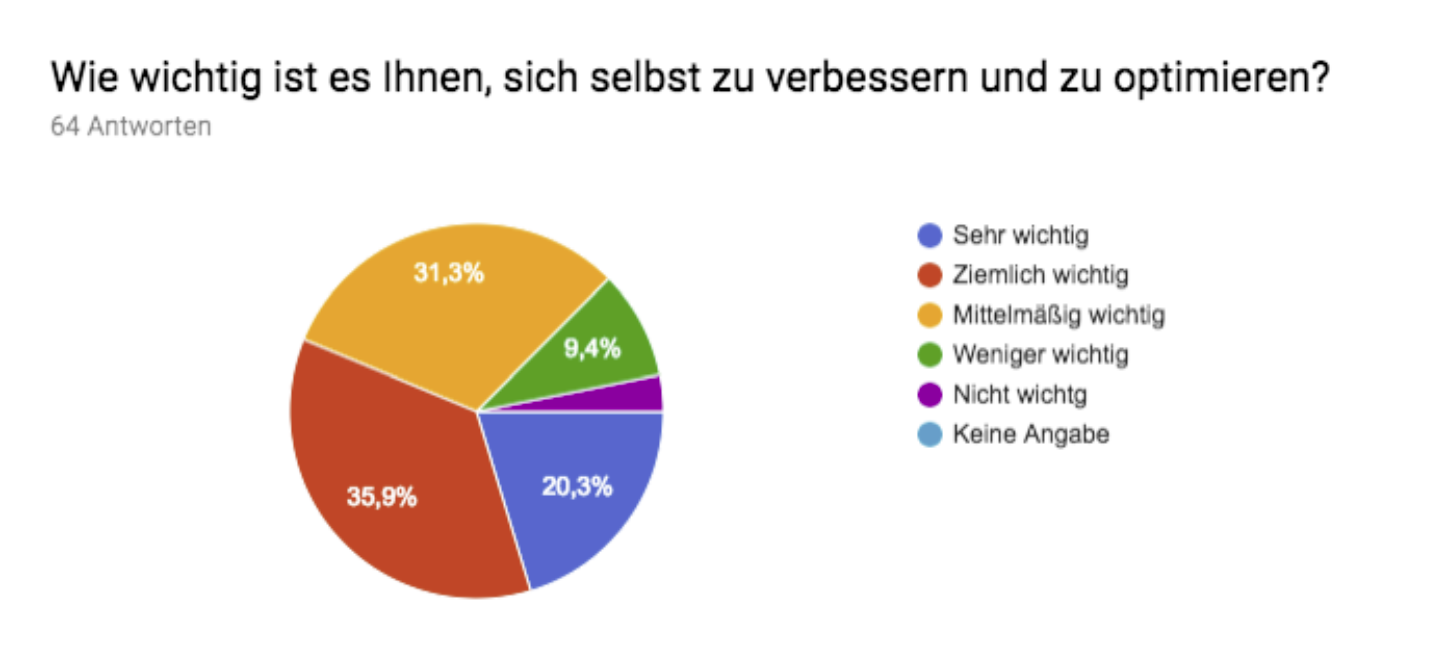
\includegraphics[width=1.0\textwidth]{src/img/kathrin1.png}
  \caption{Diagramm zu den Antworten der Frage: \enquote{Wie wichtig ist es
  Ihnen, sich selbst zu verbessern und zu optimieren?}}
  \label{img:kathrin1}
\end{figure}

Selbstoptimierung ist für 36 von 64 (56,3\%) sehr oder ziemlich wichtig, 20
mittelmäßig wichtig und für 8 (12,5\%) weniger oder nicht wichtig, wobei sich
keine Auffälligkeiten für die verschiedenen Geschlechter, Altersgruppen oder
Technikvorerfahrungen gibt.

Mit 39 Nennungen ist Bildung der stärkste Bereich, in dem die Befragten sich
verbessern, gefolgt von Sport (35) und Ernährung (29). 24 Personen geben an
sich beim Zeit- und Selbstmanagement, 21 Personen beim Sprache(n) lernen und
5 in kleinem Bereich zu optimieren.

Bei der Verwendung technischer Hilfsmittel liegt das Smartphone mit 39
Nennungen vorne, danach folgen Wearables (10) und die Sprachsteuerung (4).
Aus 8 Freitextantworten ergeben sich folgende Hilfsmittel: PC bzw. Computer,
Bücher, Fachliteratur, Meditation, Medikamente, Excel, Websites oder
Empfehlungen. 18 Befragte geben an keine Hilfsmittel zu nutzen.

Die Auswertung zur Häufigkeit der Hilfsmittelnutzung zeigt, dass drei
Antwortmöglichkeiten dominieren: mehrmals am Tag mit 14 (21,9\%), mehrmals in
einer Woche mit 17 (26,6\%) und gar nicht mit 16 (25\%).

\begin{figure}[H]
  \centering
  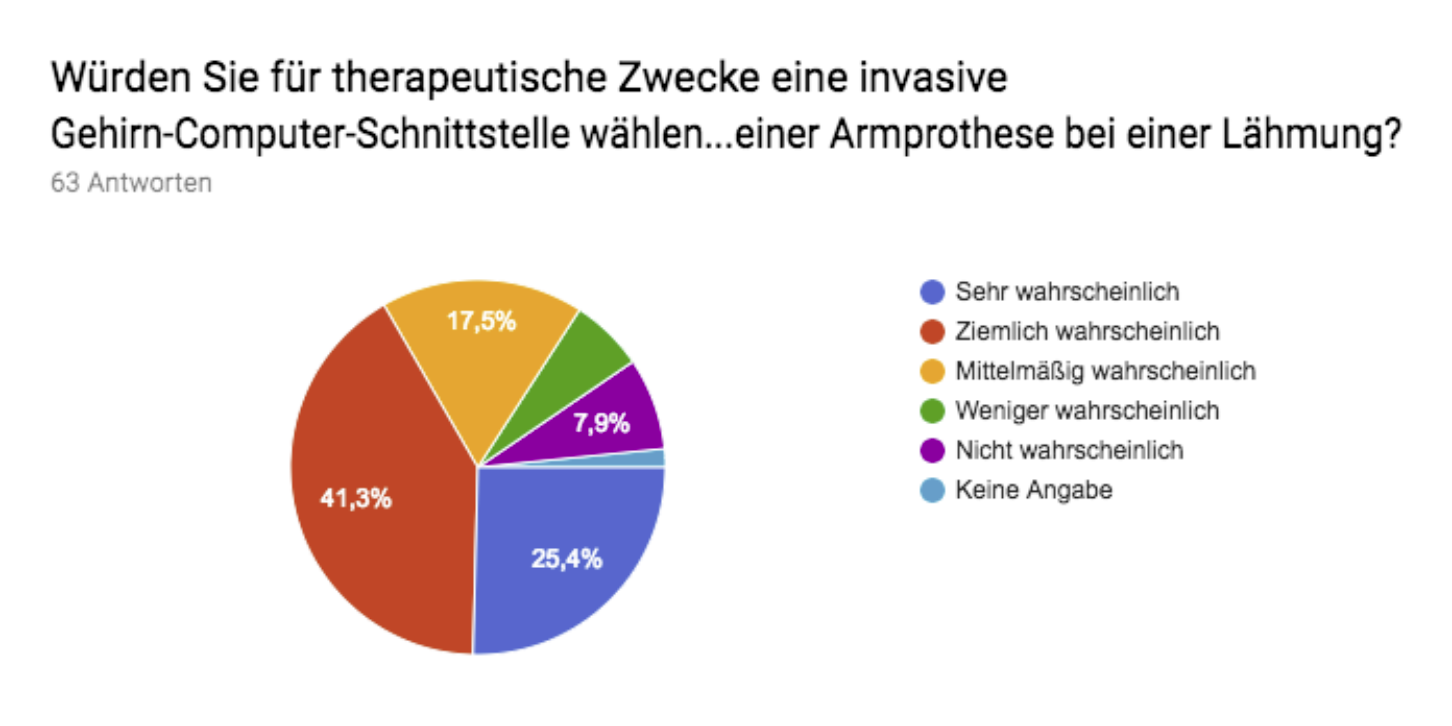
\includegraphics[width=1.0\textwidth]{src/img/kathrin2.png}
  \caption{Diagramm zu den Antworten der Frage: \enquote{Würden Sie für
  therapeutische Zwecke eine invasive Gehirn-Computer-Schnittstelle wählen
  ...?}}
  \label{img:kathrin2}
\end{figure}

Für therapeutische Zwecke würden 42 von 63 (66,7\%) sehr oder ziemlich
wahrscheinlich, eine invasive BCI wählen. Damit ist der Prozentsatz hier
höher als bei der Frage zur Selbstoptimierung, vermutlich durch den
Ausgangspunkt einer Krankheit oder Behinderung. 11 antworten mit mittelmäßig
wahrscheinlich, 9 (14,3\%) mit weniger oder nicht wichtig . Eine leichte
Abweichung gibt es bei den Geschlechtern: bei Männer sind die Angaben sehr
oder ziemlich wahrscheinlich etwas höher, 27 von 38 (71,1\%), als bei den
Frauen, 13 von 20 (65\%). Für die Altersgruppen und Technikvorerfahrungen sind
keine Unterschiede zu erkennen.

\begin{figure}[H]
  \centering
  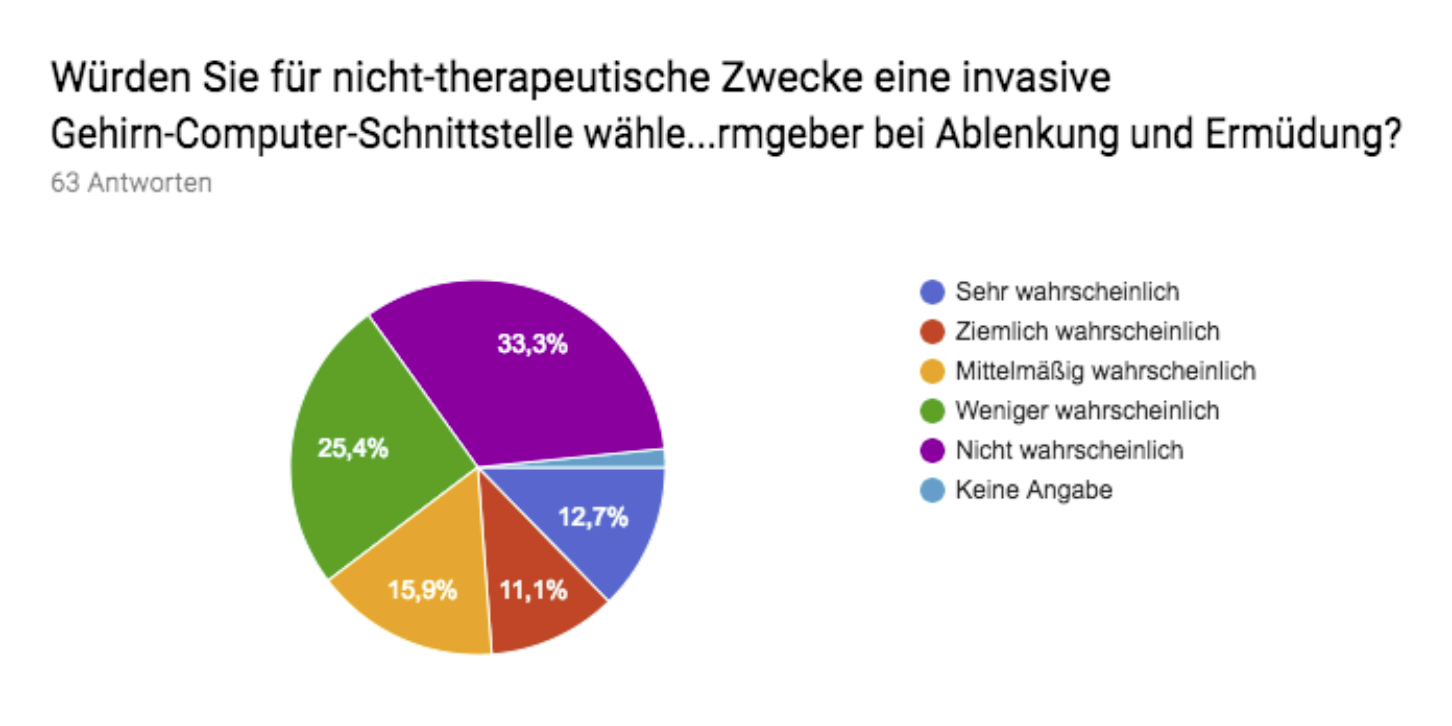
\includegraphics[width=1.0\textwidth]{src/img/kathrin3.png}
  \caption{Diagramm zu den Antworten der Frage: \enquote{Würden Sie für
  nicht-therapeutische Zwecke eine invasive Gehirn-Computer-Schnittstelle
  wählen ...?}}
  \label{img:kathrin3}
\end{figure}

Bei den Antworten zur Verwendung einer invasiven BCI für nicht-therapeutische
Zwecke zeigt sich ein fast umgekehrtes Bild, 15 von 63 (23,8\%) nennen sehr
oder ziemlich wahr- scheinlich, 10 mittelmäßig und 37 (58,7\%) weniger oder
nicht wahrscheinlich. Diese ausgeprägte Zurückhaltung variiert stark
innerhalb der Geschlechter, Altersgruppen und Technikvorerfahrungen. Männer
sind offener für die nicht-therapeutische Verwendung, 12 von 38 (31,6\%)
antworten sehr oder ziemlich wahrscheinlich. Bei Frauen schneit es große
Skepsis beim Einsatz bei einem gesunden Menschen zu geben: 14 von 20 (70\%)
sagen weniger oder nicht wahrscheinlich.

\begin{figure}[H]
  \centering
  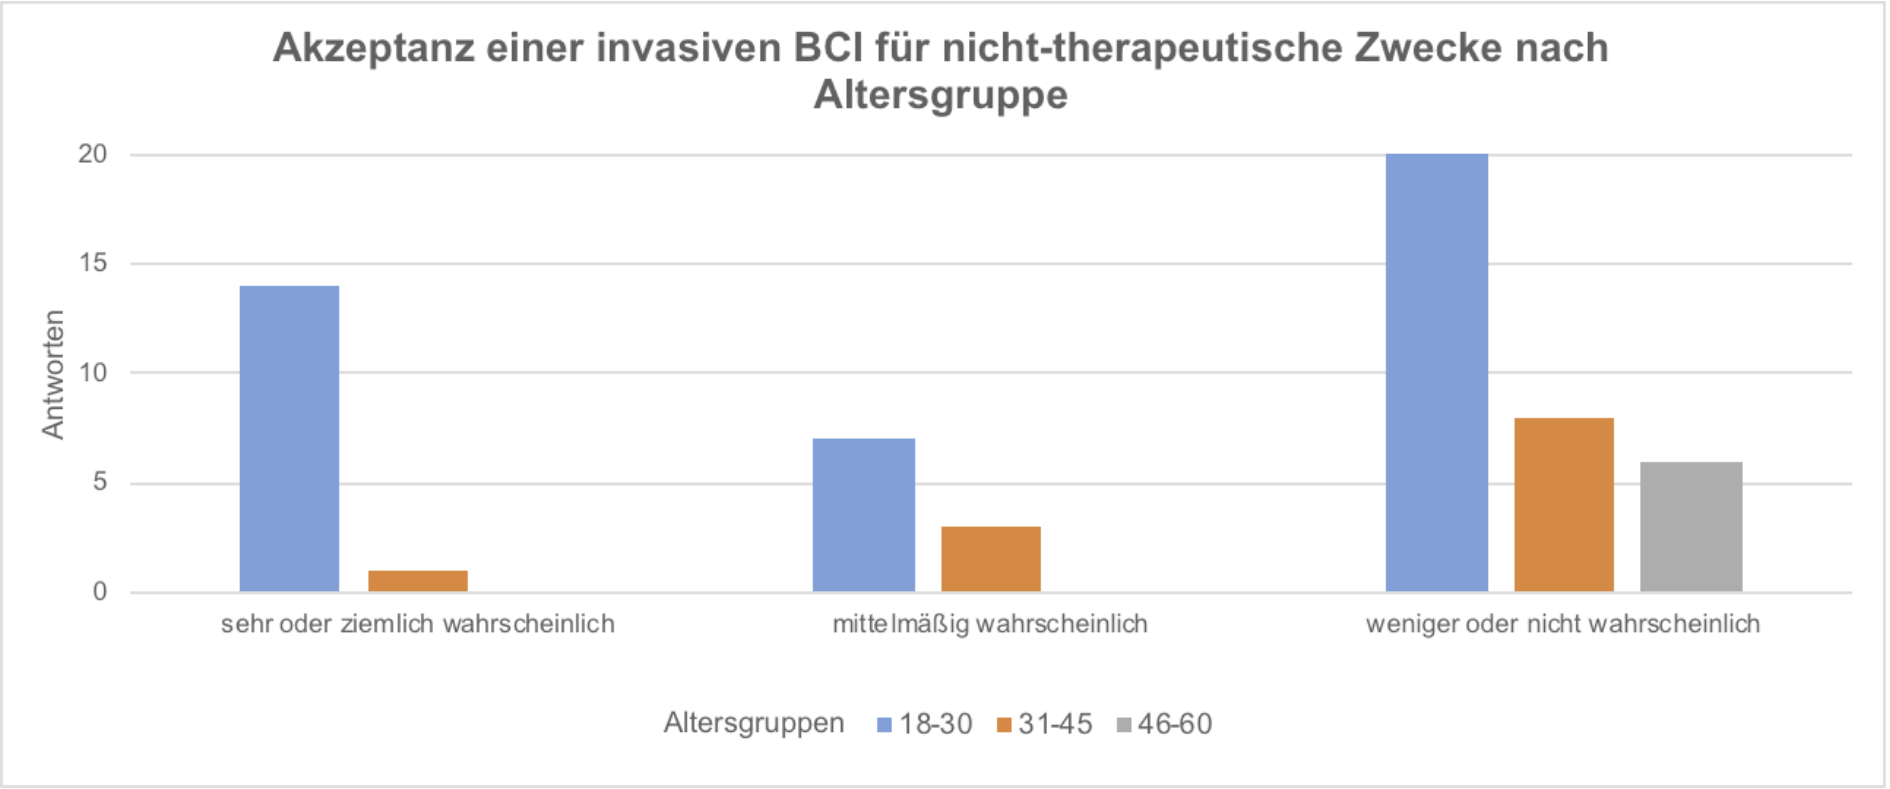
\includegraphics[width=1.0\textwidth]{src/img/kathrin4.png}
  \caption{Akzeptanz einer invasiven BCI für nicht-therapeutische Zwecke nach
  Altersgruppe}
  \label{img:kathrin4}
\end{figure}

Für die Altersgruppen lässt sich sagen, dass mit steigendem Alter die
Akzeptanz deutlich sinkt. In der Altersgruppe 46-60 ist die Basis mit 6
Antworten gering.

\begin{figure}[H]
  \centering
  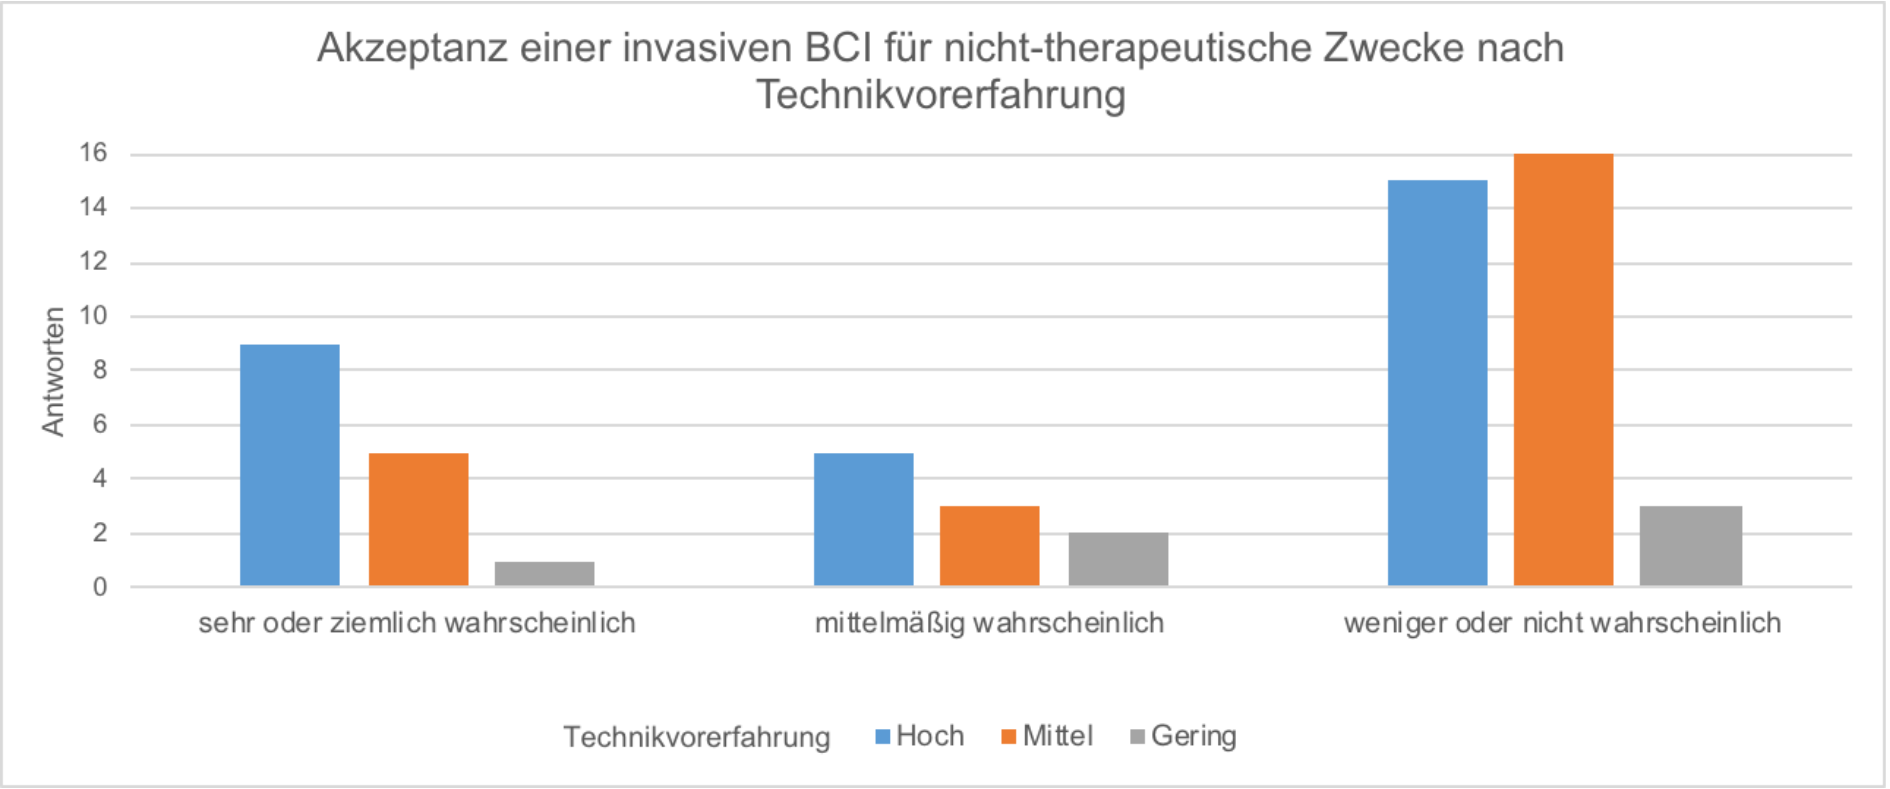
\includegraphics[width=1.0\textwidth]{src/img/kathrin5.png}
  \caption{Akzeptanz einer invasiven BCI für nicht-therapeutische Zwecke nach
  Technikvorerfahrung}
  \label{img:kathrin5}
\end{figure}

Ebenso korreliert die Akzeptanz mit der Technikvorerfahrung. Für die
Technikvorerfahrung \enquote{Gering} ist die Basis mit 6 Antworten klein.
Die etwas komplexere Frage zur Risikobewertung haben 62 Personen beantwortet.
Die Risiken werden absteigend nach den Nennungen für sehr hohes oder hohes
Risiko aufgeführt. Als stärkstes Risiko wird der Missbrauch von im Gehirn
erhobenen Daten angesehen, 43 (69,4\%) geben dafür an. Die Klärung der
Verantwortung bei Schädigung Dritter und das Risiko von Ungerechtigkeit sind
mit 38 bzw. 37 Nennungen (61,3\% bzw. 60,0\%) ähnlich bewertet. Bei den
medizinischen Risiken sind es 32 Antworten (51,6\%), allerdings ist der Wert
für das mittelmäßige Risiko mit 21 hier hoch. Danach folgt das Risiko zur
Ausgrenzung von Individuen und Gruppen, hier sind es 29 (46,8\%). Am wenigsten
bedrohlich werden die unbefugte Steuerung von Außen und die Veränderung der
eigenen Persönlichkeit wahrgenommen, 23 bzw. 21 gaben dies an (37,0\% bzw.
33.9\%). Bei beiden ist sind die Nennung für das mittelmäßige Risiko mit 24
bzw. 22 stark ausgeprägt.

\subsection{Zusammenfassung}
\label{subsec:kathrin_zusammenfassung}
Zu Human Enhancement und der Verwendung von BCIs gibt es eine Vielzahl von
ethischen Aspekten. Deren Reflektion kann helfen, das BCIs eine breite
Akzeptanz in der Gesellschaft finden. Die Analyse der Umfragewerte hat
ergeben, dass der befragte Personenkreis Selbstoptimierung zu 50\% als
ziemlich oder sehr wichtig bewertet und nur für wenige einen kleinen oder gar
keinen Stellenwert hat. Noch höher ist die Akzeptanz von BCIs zu
therapeutischen Zwecken mit 67\%, vermutlich aus der Not einer Krankheit oder
Behinderung heraus. Bei der Verwendung von BCIs bei gesunden Menschen zur
Selbstoptimierung dreht sich das Bild, nur noch 24\% haben eine bejahende
Einstellung zur Verwendung. Bei dieser Frage gibt es große Unterschiede
innerhalb der Geschlechter, Altersgruppen und Technikvorerfahrungen.

\newpage
\printbibliography[heading=bibintoc]

\end{document}
